<<<<<<< HEAD
\subsection{Bussluse som løsningforslag for et tryggere område i Nytorv/Østerågade}
\label{bussluselosningforslag}
=======
\subsection{Bussluse}
\label{bussluse}

I dette afsnit er forskellen på bus sluserne beskrevet, da de har forskellig udformning. Der overvejes et løsningforslag, som kan bruges i området på Nytorv/Østerågade. Forslaget vil udmunde beskrivelse og tegninger for, hvordan en løsning kan se ud på Nytorv/Østerågade og gennem Boulevarden.
>>>>>>> cecf2882df1ee084eb1246487e3544cbc3e71c22

I Aalborg har man tidligere anvendt bus sluser på mange steder, som ved skoler og områder med stilleveje. På Nytorv/Østerågade ligger mange restauranter, shoppingfaciliteter og cafeér, og som nævnt tidligere, er der mange mennesker, som færdes i området. Samtidig er der forbud af gennemkørsel af privatbiler i området, men det er aldrig blevet respekteret fuldt ud, da mere end 3000 biler passerer Østerågade hver dag. (3000 biler passerer hverdag Østerågade som står i P1 projektkatalog under Nytorv/Østerågade - Problemstilling)

Busgrav og hæve sænke pullerter er forskellige måder at lave bus sluser på.

En busgrav er ofte et hul eller en forhøjning i midten af vejbanen. I busgrave er bredden på hullet tilpasset bredden på bussens hjulpar. Dvs. at kun busser kan passere slusen, hvorimod privatbiler, med mindre bredde mellem hjulparene, vil falde i hullet. På hver side af hullet, er der ofte forhøjninger så privatbiler går i stykker, hvis de prøver at kører højre eller venstre om slusen. 
\\\\
Hæve sænke pullerter består af flere cylindre -pneumatik med en bestemt afstand mellem hver cylinder. Standart størrelsen som f. eks. 250 x 500 mm (diameter gange højde) eller 200 x 500 mm osv. Produktet kan styres ved hjælp af tidsstyring og/eller fjernbetjening ( http://www.g9-se.se/regulering-i-byrum.html ). Når en bus nærmer sig mod cylinderne, så sænkes cylinderne pr. automatik. 

\begin{figure}[htbp]
  \centering
  \begin{adjustbox}{max width=\textwidth}
    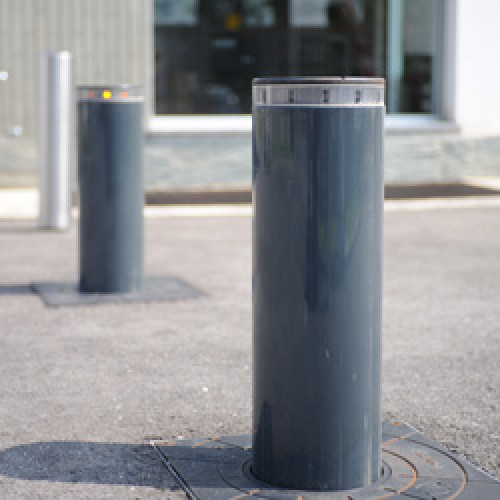
\includegraphics{figures/Billederogfigur/1.jpg}
 \end{adjustbox}
  \caption{byrum billede %Billede fra %http://www.g9.dk/media/blfa_files/Luxor_pullert.pdf}
   \label{fig:byrum %Billede fra %http://www.g9.dk/media/blfa_files/Luxor_pullert.pdf}
\end{figure}

        
        %Billede fra %http://www.g9.dk/media/blfa_files/Luxor_pullert.pdf

\subsection{Bussluserne i Nytorv/Østerågade}
\label{bussluseinytorv}                                           
                                           
                                           
Hæve sænke pullerter som cylinder -pneumatik udføres som følgende. Ved Stranden med retning mod Østerågade kan laves cylinder -pneumatik. Privatbilister kan svinge før bus slusen og finde parkering til deres biler, og gå på Østerågade området. 
                                        
\subsubsection{Bussluserne i Nytorv/Østerågade}
\label{subs:buslusnytorv}
{Bussluserne i Nytorv/Østerågade}
\label{sub:}
\begin{figure}[htbp]
  \centering
  \begin{adjustbox}{max width=\textwidth}
    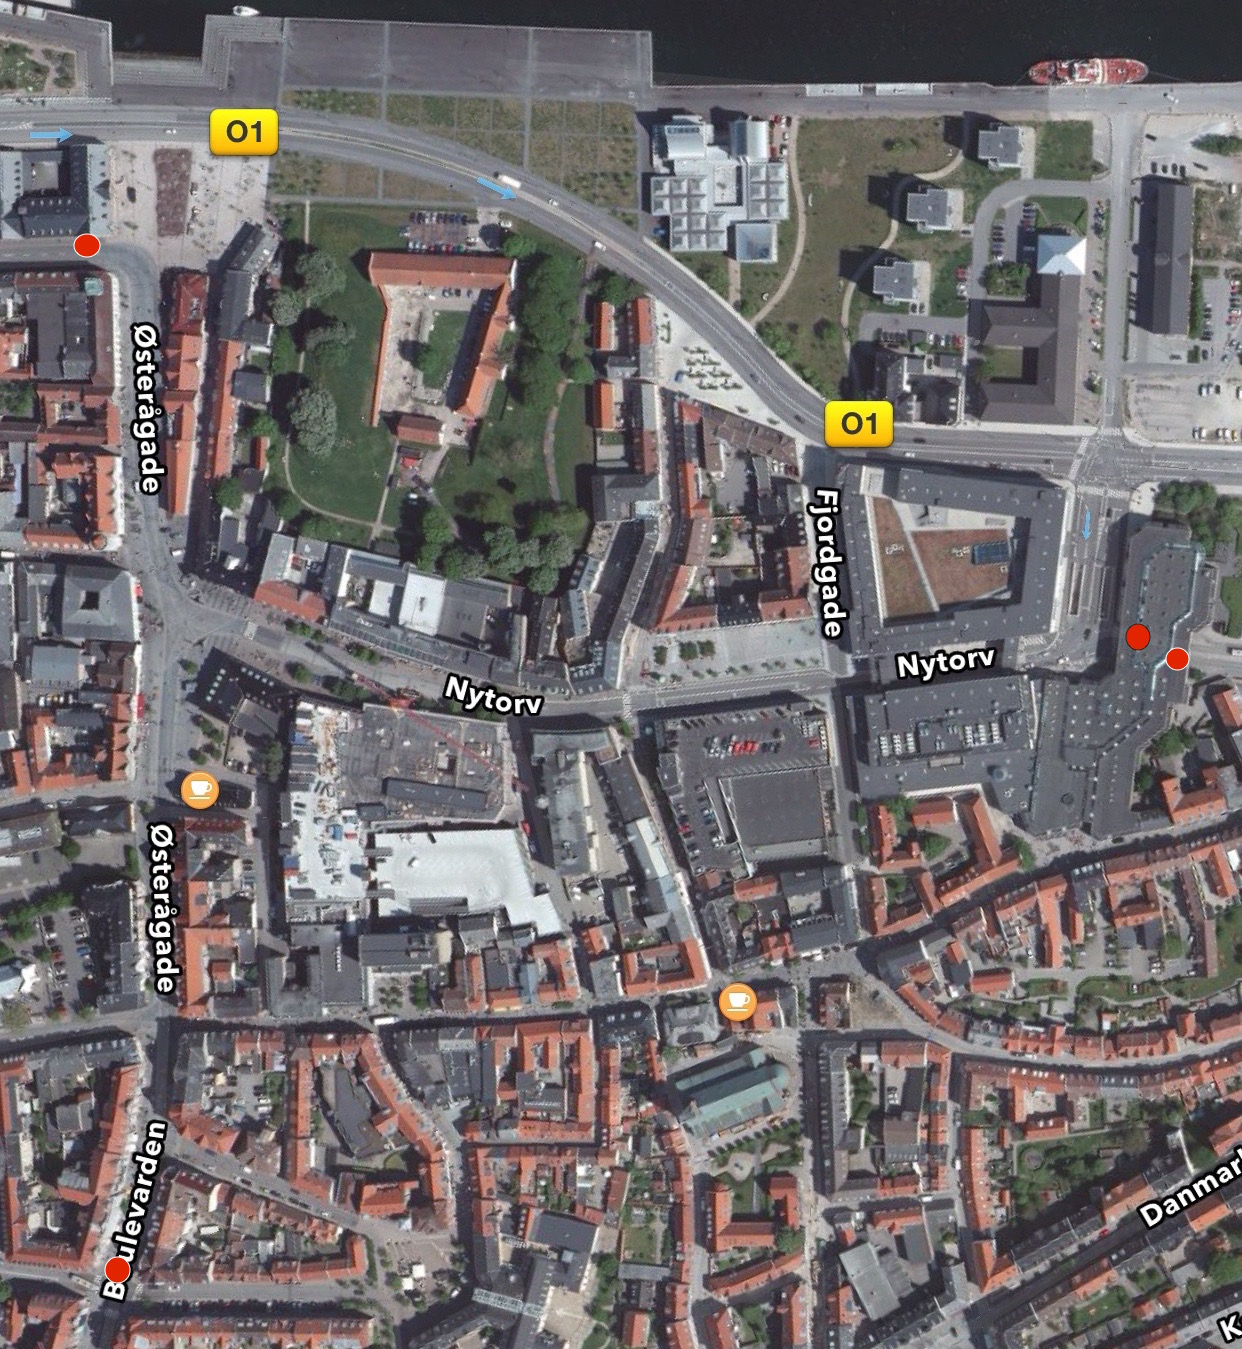
\includegraphics{figures/Billederogfigur/2.jpg}
 \end{adjustbox}
  \caption{ Fotograf af Rong’s mobil, og udarbejder Rong Liu}
   \label{fig: Fotograf af Rong}
\end{figure}
                                        
Under Aalborg biblioteket er der skilte med indkørsel forbudt for privatbiler, men de kører alligevel igennem. Her kan der ligeledes placeres cylinder - pneumatik under biblioteket. Dermed undgår at privatbiler kører denne vej. Privatbiler kan parkere i Friis’s parkeringshus, i Føtex eller hos Salling.                         
                                                   
\begin{figure}[htbp]
  \centering
  \begin{adjustbox}{max width=\textwidth}
    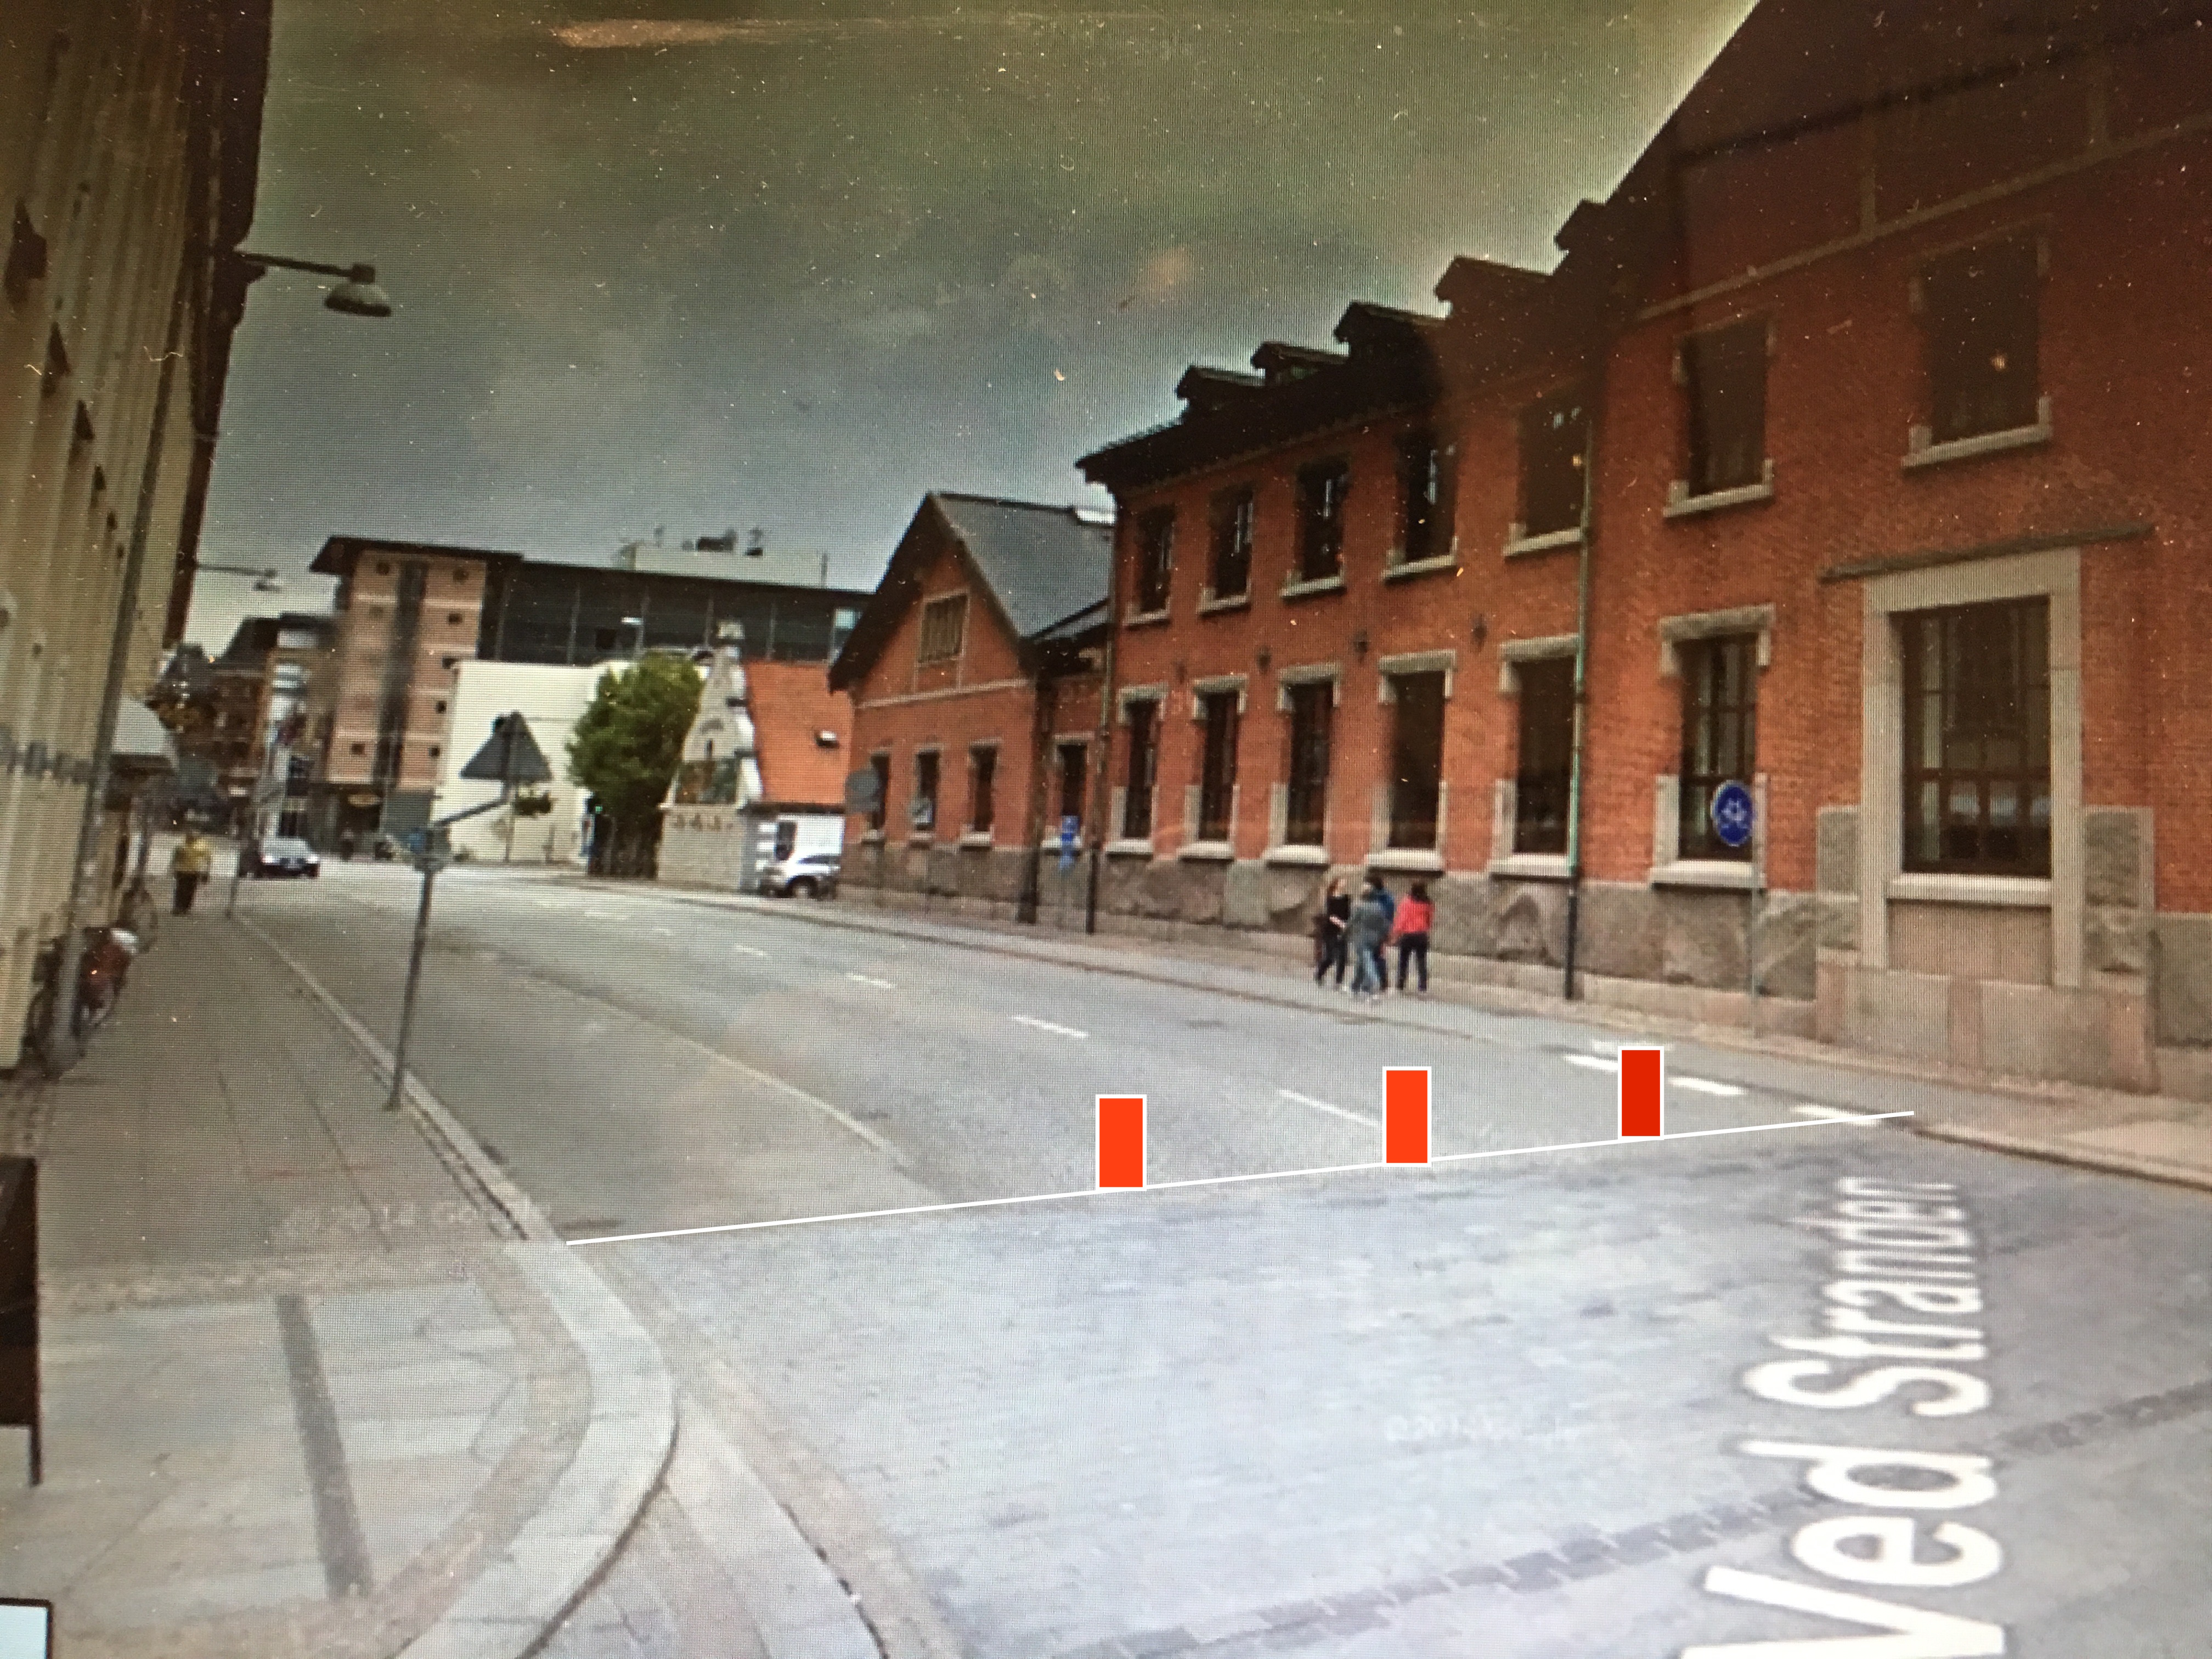
\includegraphics{figures/Billederogfigur/3.jpg}
 \end{adjustbox}
  \caption{ Fotograf af Rong’s mobil, og udarbejder Rong Liu}
   \label{fig: Fotograf af Rong}
\end{figure}
                                                   

På Boulevarden kan der placeres cylinder - pneumatik. På dette sted er der ligeledes indkørsel forbudt for privatbiler, men ikke alle overholder denne skiltning. Privatbiler kan svinge før korsvej på Vingårdsgade og parkeringer deres biler ved Budolfi Kirke eller på Budolfi Plads. 
                                                
\begin{figure}[htbp]
  \centering
  \begin{adjustbox}{max width=\textwidth}
    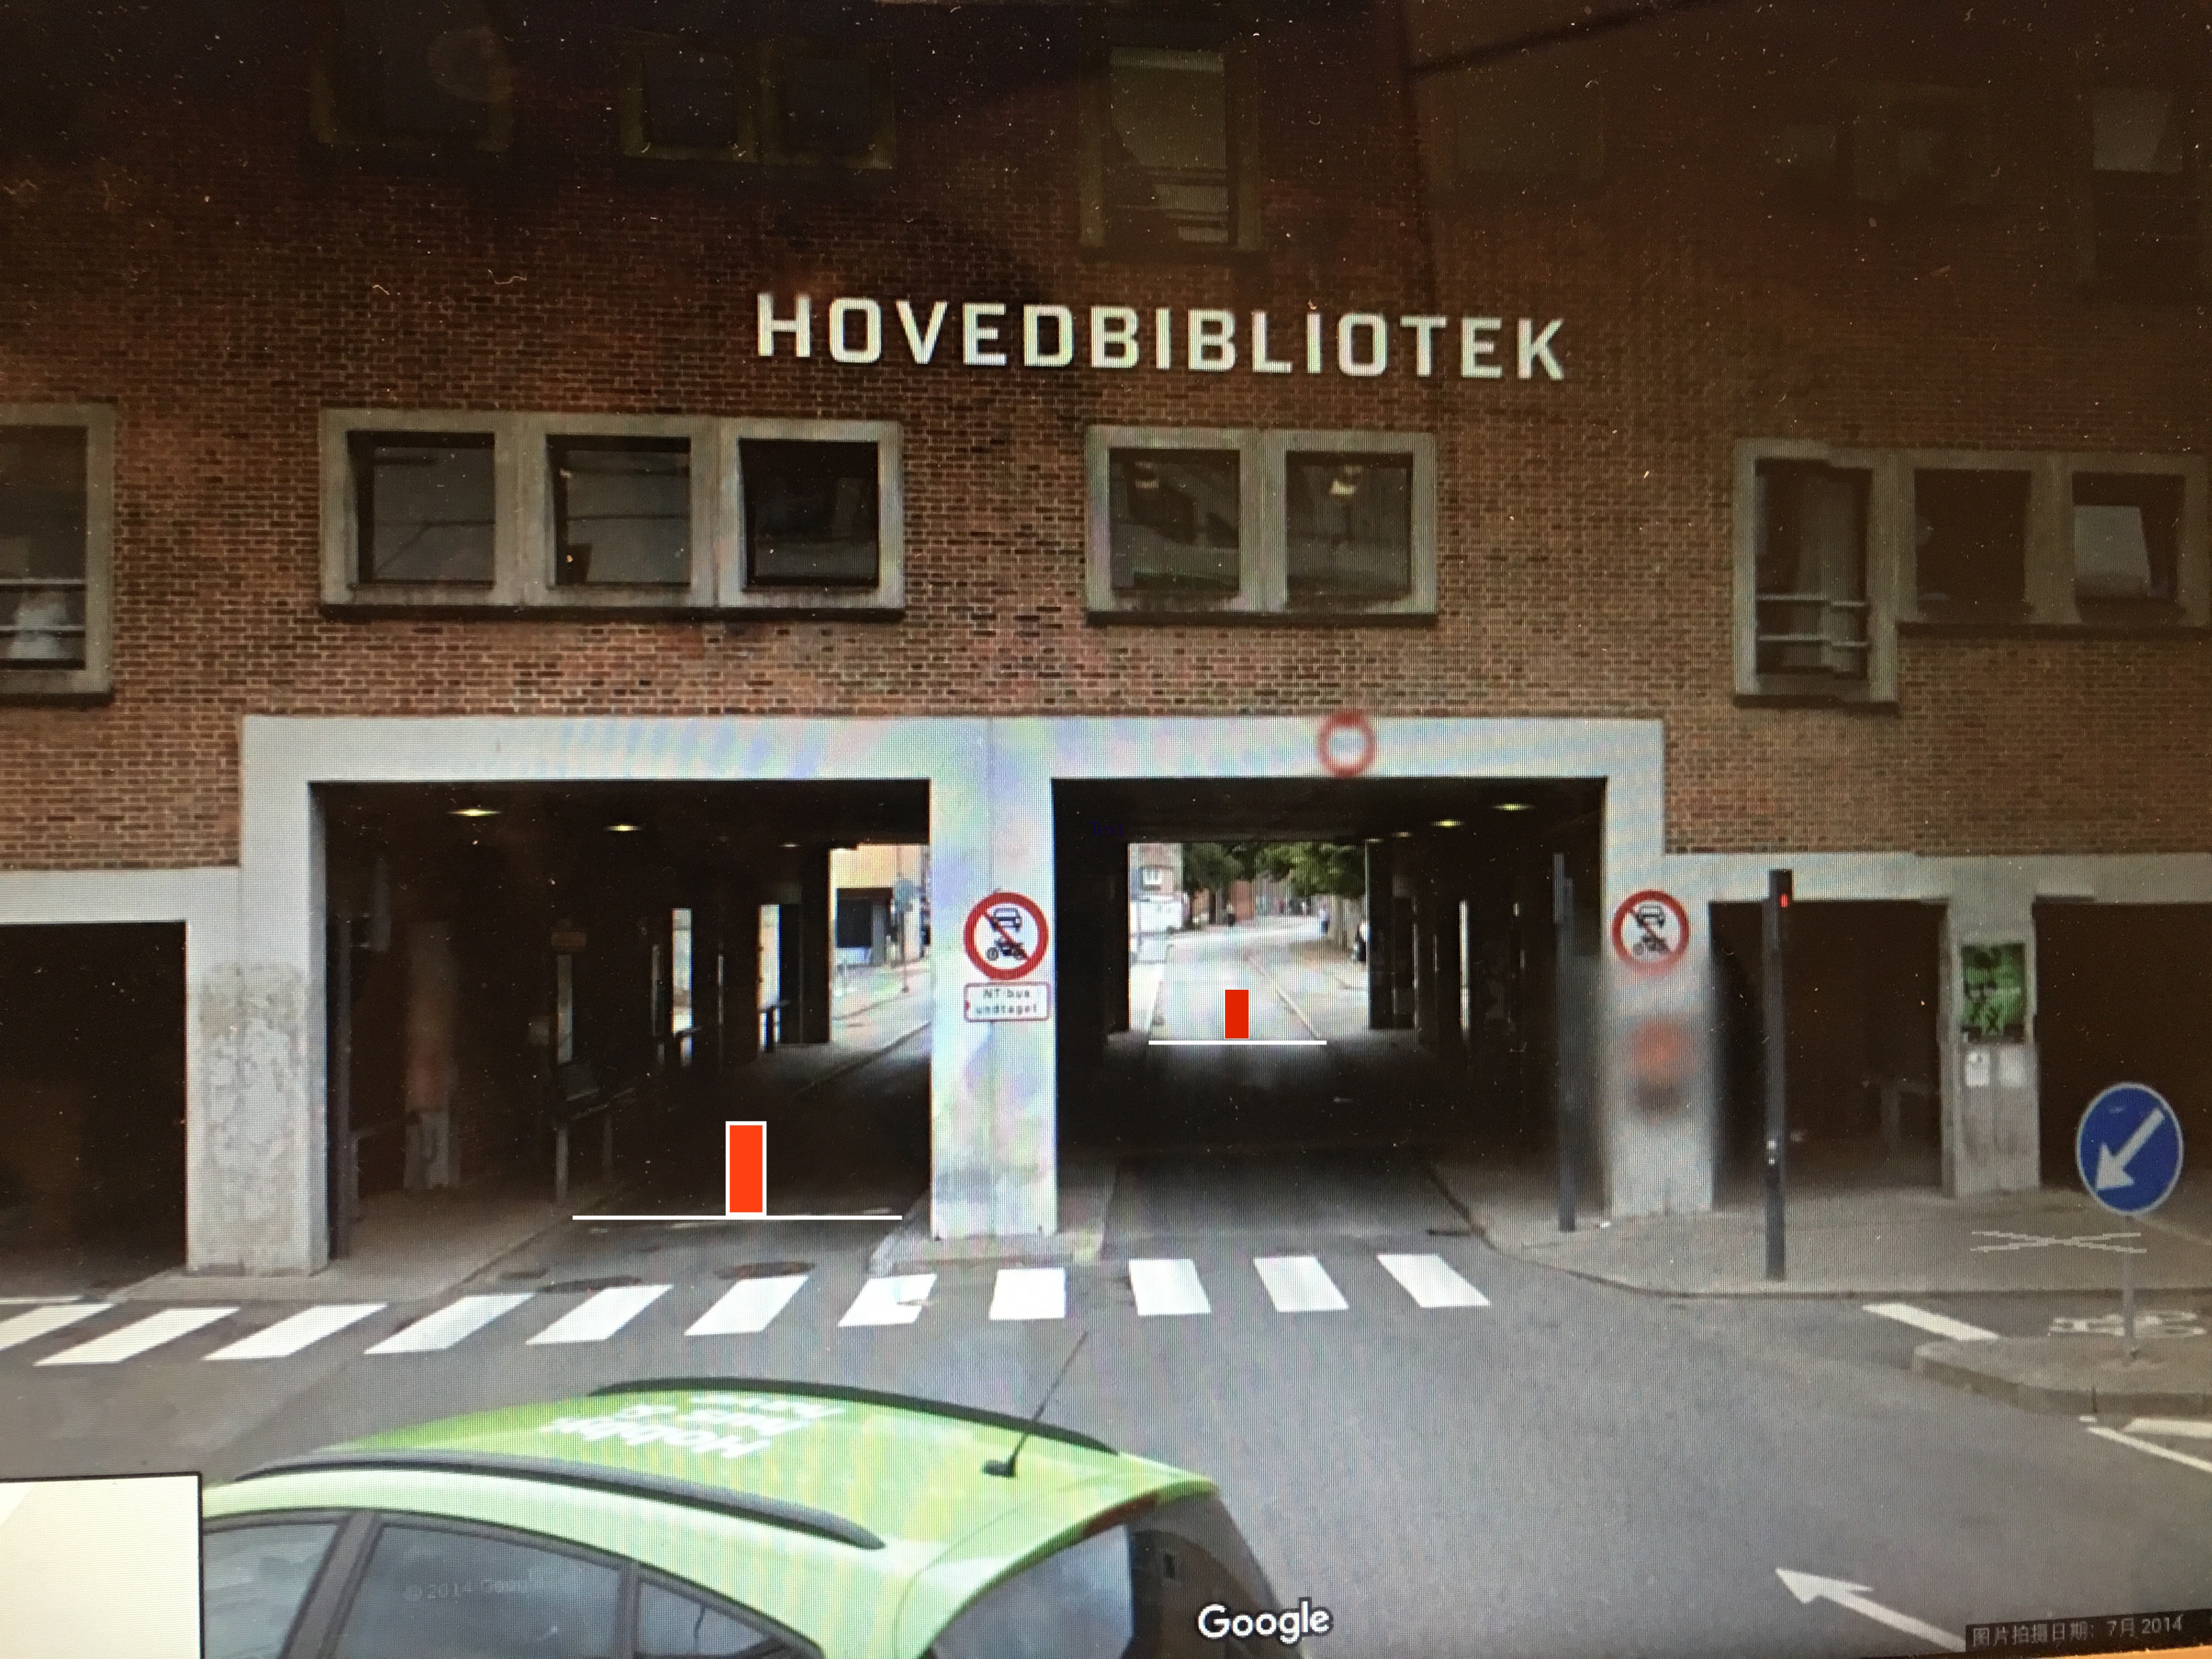
\includegraphics{figures/Billederogfigur/4.jpg}
 \end{adjustbox}
  \caption{ Fotograf af Rong’s mobil, og udarbejder Rong Liu}
   \label{fig: Fotograf af Rong}
\end{figure}

                                       

\begin{figure}[htbp]
  \centering
  \begin{adjustbox}{max width=\textwidth}
    \includegraphics{figures/Billederogfigur/5.jpg}
 \end{adjustbox}
  \caption{ Fotograf af Rong’s mobil, og udarbejder Rong Liu}
   \label{fig: Fotograf af Rong}
\end{figure}
>>>>>>> cecf2882df1ee084eb1246487e3544cbc3e71c22
Disse løsninger er et forsøg på at gøre Nytorv/Østerågade delvist privatbilfrit. Der er derfor kun tilladt for busser og cyklister. Det må og vil give mere sikkerhed til fodgængere.
~\\\\
Bus sluser som hæve sænke pullerter er mere praktisk og vil forhindre gennemkørsel af privatbiler, således kun busser kan køre igennem. Hermed undgås privatbilstrafik inde i området. Hæve sænke pullerter vil aldrig skade biler, ligesom bus grave vil gøre, og fodgængere og cyklister vil heller ikke falde i “hullet”. Det vil give et tryggere område for cyklisterne og fodgængerne.
~\\\\
Men hæve sænke pullerter har den ulempe i forhold til busgrave, at de drives ved hjælp af elektricitet og der skal udtænkes en særlig adgangskontrol til dem som skal have adgang indenfor området. Det vil sige, at ved at vælge hæve sænke pullerter vil der være omkostninger til strøm og vedligehold og til dels administration mht. hvem der skal have permanent adgang og til dem der måske bare skal indenfor området en enkelt gang. Busgrave vil ikke forbruge noget energi, men det er ikke hensigtsmæssigt, at have “fordybninger/huller “ hvor der færdes fodgænger og cyklister.
